\documentclass[t]{beamer}

% Load general definitions
% Preamble file - general definitions, package loading, etc.

%=================================
% Load packages
\usepackage{amssymb,amsmath}
\usepackage{graphicx}
\usepackage{url}
\usepackage{tikz}
\usetikzlibrary{mindmap,trees,arrows}
\usepackage{fancyvrb}
\usepackage[portuguese]{babel} 
\usepackage[utf8]{inputenc}
\usepackage{subfigure}
\usepackage{times}
\usepackage[T1]{fontenc}
\usepackage{cancel}
\usepackage{color}
\usepackage{listings}
\usepackage[document]{ragged2e}

%=================================
% Set mode
\mode<presentation>
{
	\usetheme{Madrid}
	\usecolortheme{structure}
	\useoutertheme{infolines}
	\setbeamercovered{invisible}
}

% Get rid of nav bar
\beamertemplatenavigationsymbolsempty

% Insert frame number at bottom of the page.
\usefoottemplate{\hfil\tiny{\color{black!90}\insertframenumber}} 

%=================================
% Define new commands

\newcommand\Real{{\mathbb{R}}}
%\newcommand{\vi}{\vspace{0.6\baselineskip}}
%\newcommand{\goodgap}{\hspace{\subfigtopskip}\hspace{\subfigbottomskip}}


% Equation environments
\newcommand{\beq}{\begin{equation}}
\newcommand{\eq}{\end{equation}}
\newcommand{\beqs}{\begin{equation*}}
\newcommand{\eqs}{\end{equation*}}
\newcommand{\beqn}{\begin{eqnarray}}
\newcommand{\eqn}{\end{eqnarray}}
% Bold variables
\newcommand{\mbf}[1]{\ensuremath{\mathbf{#1}}}
% Itemization
\newcommand{\bitem}{\begin{itemize}}
\newcommand{\eitem}{\end{itemize}}
\newcommand{\spitem}{\vskip 1em\item}
\newcommand{\bitems}{\begin{itemize}\item}
\newcommand{\benums}{\begin{enumerate}\item}
\newcommand{\eenum}{\end{enumerate}}
% color blocks
\newenvironment{colorblock}[2]{%
\setbeamercolor{block title}{#2}
\begin{block}{#1}}{\end{block}}
% Vertical spacing
\newcommand{\vone}{\vskip 1em}
\newcommand{\vhalf}{\vskip .5em}
% Frame environments
\newenvironment{ftst}[3][t]{%
\begin{frame}{environment=ftst,#1}
\frametitle{#2}
\framesubtitle{#3}}{\end{frame}}
\newenvironment{ftstf}[2]{
\begin{frame}[fragile,environment=ftstf]
\frametitle{#1}
\framesubtitle{#2}}{\end{frame}}
% colors
\definecolor{MyGray}{rgb}{0.5,0.5,0.5}
\definecolor{MyDBGray}{rgb}{0.1,0.1,0.4}
\definecolor{darkgreen}{rgb}{0,0.4,0}
\definecolor{black}{rgb}{0,0,0}
\def\defn#1{{\color{red} #1}}
% Footnote
\renewcommand{\thefootnote}{\alph{footnote}}
% Relaxed footnotes
\newcommand{\lfr}[1]{\let\thefootnote\relax\footnote{\tiny #1}}
% Verbatim environment - using FANCYVRB package
\DefineVerbatimEnvironment%
{rcode}{Verbatim}
{fontsize=\scriptsize}
% Verbatim environment - using LISTINGS package
%\lstnewenvironment{rcode} {\lstset{	language = R,
%									basicstyle = \scriptsize\ttfamily,
%									showspaces = false,
%									showstringspaces = false,
%									showtabs = false,
%									keywordstyle = \color{black}\bfseries,
%									commentstyle = \color{darkgreen},
%									numbers = none,
%									otherkeywords={	<-,
%													ggplot,
%													geom_boxplot,
%													facet_grid,
%													shapiro.test,
%													fligner.test,
%													glht,
%													with},
%									deletekeywords={data,
%													model,
%													residuals,
%													c,
%													axis,
%													default,
%													labels,
%													qq.text}}}%
%{}

% Specific definitions
\title[]{Algoritmos e Estruturas de Dados III}
\subtitle[]{Introdução à Teoria dos Grafos}
\author[]{Patrícia Lucas\\{\footnotesize }}
\institute{Bacharelado em Sistemas de Informação \\ IFNMG  - Campus Salinas}
\date{\scriptsize Salinas\\Dezembro 2020}

\begin{document}

% cover page
\setbeamertemplate{footline}{}
\begin{frame}

\begin{center}
\includegraphics[width=.15\textwidth]{}
\end{center}
  \titlepage
  \begin{tikzpicture}[remember picture,overlay]
  \node[anchor=south east,xshift=-5pt,yshift=5pt] at (current page.south east) {\tiny Versão 1.2020};
  \node[anchor=south west,yshift=0pt] at (current page.south west) {
\includegraphics[width=.25\textwidth]{Logos/salinas_horizontal_jpg.jpg}};
  \end{tikzpicture}  
\end{frame}

% Main slides
\begin{ftst}{Conceito}{Teoria dos grafos}

\begin{itemize}
    \item A teoria dos grafos é um subconjunto da matemática discreta. 
    \item Um grafo é usado para modelar coisas que têm relações com outras coisas - essa definição vaga sugere a enorme flexibilidade dos grafos na resolução de problemas. 
    \item O notável poder da teoria dos grafos foi usado para resolver problemas em praticamente todas as áreas.
\end{itemize}

\end{ftst}

%=====

\begin{ftst}{Terminologia}{Teoria dos grafos}

Um grafo simples $G =(V,E)$ consiste de um conjunto não vazio $V$ de vértices e um conjunto que pode ou não ser vazio $E$ de arestas, cada aresta sendo um conjunto de dois vértices $(v_i, v_j)$ a partir de $V$, sendo $(v_i,v_j)=(v_j,v_i)$. \\
\vone
O número de vértices e arestas é denotado por $|V|$ e $|E|$, respectivamente.

\centering 

\tikzset{every picture/.style={line width=0.75pt}} %set default line width to 0.75pt        

\begin{tikzpicture}[x=0.75pt,y=0.75pt,yscale=-1,xscale=1]
%uncomment if require: \path (0,125); %set diagram left start at 0, and has height of 125

%Shape: Ellipse [id:dp56526211521717] 
\draw  [fill={rgb, 255:red, 0; green, 0; blue, 0 }  ,fill opacity=1 ] (46.35,48.98) .. controls (46.35,44.17) and (50.56,40.28) .. (55.75,40.28) .. controls (60.94,40.28) and (65.15,44.17) .. (65.15,48.98) .. controls (65.15,53.79) and (60.94,57.69) .. (55.75,57.69) .. controls (50.56,57.69) and (46.35,53.79) .. (46.35,48.98) -- cycle ;
%Shape: Ellipse [id:dp704999339935936] 
\draw  [fill={rgb, 255:red, 0; green, 0; blue, 0 }  ,fill opacity=1 ] (100.36,99.41) .. controls (100.36,94.6) and (104.57,90.71) .. (109.76,90.71) .. controls (114.95,90.71) and (119.15,94.6) .. (119.15,99.41) .. controls (119.15,104.22) and (114.95,108.11) .. (109.76,108.11) .. controls (104.57,108.11) and (100.36,104.22) .. (100.36,99.41) -- cycle ;
%Shape: Ellipse [id:dp18766605151664573] 
\draw  [fill={rgb, 255:red, 0; green, 0; blue, 0 }  ,fill opacity=1 ] (105.31,49.67) .. controls (105.31,44.86) and (109.52,40.97) .. (114.71,40.97) .. controls (119.9,40.97) and (124.11,44.86) .. (124.11,49.67) .. controls (124.11,54.48) and (119.9,58.37) .. (114.71,58.37) .. controls (109.52,58.37) and (105.31,54.48) .. (105.31,49.67) -- cycle ;
%Shape: Ellipse [id:dp860106873164983] 
\draw  [fill={rgb, 255:red, 0; green, 0; blue, 0 }  ,fill opacity=1 ] (74.61,67.65) .. controls (74.61,62.84) and (78.82,58.94) .. (84.01,58.94) .. controls (89.2,58.94) and (93.4,62.84) .. (93.4,67.65) .. controls (93.4,72.45) and (89.2,76.35) .. (84.01,76.35) .. controls (78.82,76.35) and (74.61,72.45) .. (74.61,67.65) -- cycle ;
%Shape: Ellipse [id:dp9624212908786325] 
\draw  [fill={rgb, 255:red, 0; green, 0; blue, 0 }  ,fill opacity=1 ] (22.17,75.88) .. controls (22.17,71.07) and (26.38,67.17) .. (31.57,67.17) .. controls (36.76,67.17) and (40.96,71.07) .. (40.96,75.88) .. controls (40.96,80.68) and (36.76,84.58) .. (31.57,84.58) .. controls (26.38,84.58) and (22.17,80.68) .. (22.17,75.88) -- cycle ;
%Shape: Ellipse [id:dp666723248449479] 
\draw  [fill={rgb, 255:red, 0; green, 0; blue, 0 }  ,fill opacity=1 ] (76.05,15.56) .. controls (76.05,10.75) and (80.26,6.85) .. (85.45,6.85) .. controls (90.64,6.85) and (94.85,10.75) .. (94.85,15.56) .. controls (94.85,20.37) and (90.64,24.26) .. (85.45,24.26) .. controls (80.26,24.26) and (76.05,20.37) .. (76.05,15.56) -- cycle ;
%Shape: Ellipse [id:dp9741887195317744] 
\draw  [fill={rgb, 255:red, 0; green, 0; blue, 0 }  ,fill opacity=1 ] (29.06,13.82) .. controls (29.06,9.01) and (33.27,5.11) .. (38.46,5.11) .. controls (43.65,5.11) and (47.86,9.01) .. (47.86,13.82) .. controls (47.86,18.62) and (43.65,22.52) .. (38.46,22.52) .. controls (33.27,22.52) and (29.06,18.62) .. (29.06,13.82) -- cycle ;
%Shape: Ellipse [id:dp5101164697169429] 
\draw  [fill={rgb, 255:red, 0; green, 0; blue, 0 }  ,fill opacity=1 ] (5,40.28) .. controls (5,35.47) and (9.21,31.57) .. (14.4,31.57) .. controls (19.59,31.57) and (23.8,35.47) .. (23.8,40.28) .. controls (23.8,45.08) and (19.59,48.98) .. (14.4,48.98) .. controls (9.21,48.98) and (5,45.08) .. (5,40.28) -- cycle ;
%Straight Lines [id:da6271899558210341] 
\draw [fill={rgb, 255:red, 0; green, 0; blue, 0 }  ,fill opacity=1 ]   (29.55,71) -- (17.14,46.21) ;
%Straight Lines [id:da2230066147300016] 
\draw [fill={rgb, 255:red, 0; green, 0; blue, 0 }  ,fill opacity=1 ]   (19.9,32.51) -- (30.92,20.12) ;
%Straight Lines [id:da5606460186184359] 
\draw    (47.47,10.33) -- (76.42,11.64) ;
%Straight Lines [id:da6611820119232676] 
\draw    (38.51,69.7) -- (51.6,55.35) ;
%Straight Lines [id:da8708544360856261] 
\draw    (61.25,42.3) -- (79.86,22.08) ;
%Straight Lines [id:da4619727420957742] 
\draw    (89.51,20.12) -- (111.57,45.56) ;
%Straight Lines [id:da7644501958337031] 
\draw    (85.45,15.56) -- (84.01,67.65) ;
%Straight Lines [id:da22348802745324092] 
\draw    (31.57,75.88) -- (109.76,99.41) ;
%Straight Lines [id:da6696267389895008] 
\draw    (84.01,67.65) -- (109.76,99.41) ;
%Straight Lines [id:da6177319913365642] 
\draw    (114.71,49.67) -- (109.76,99.41) ;




\end{tikzpicture}
Exemplo: Grafo com $|V| = 8$ e $|E| = 10$

\end{ftst}

%=====

\begin{ftst}{Aplicações}{Teoria dos grafos}
\justifying
\begin{itemize}
    \item O projeto do sistema de água municipal utiliza a teoria dos grafos para modelar o fluxo de água para garantir que os requisitos de pressão sejam atendidos.
    \item Redes sociais como Facebook e Twitter usam a teoria dos grafos para sugerir amigos e vender anúncios.
    \item A Netflix usa a teoria dos grafos para recomendar filmes.
    \item O Google Maps usa a teoria dos grafos para encontrar o caminho mais curto da sua casa até o seu destino.
    \item A infraestrutura da Internet se baseia na teoria dos grafos para rotear seu tráfego de nó em nó na infraestrutura física da internet.
    \item Os engenheiros de videogame usam a teoria dos grafos para direcionar os NPCs (personagens não jogadores) por seus mundos virtuais.
\end{itemize}

\end{ftst}

%=====

\begin{ftst}{Aplicações}{Teoria dos grafos}

\centering
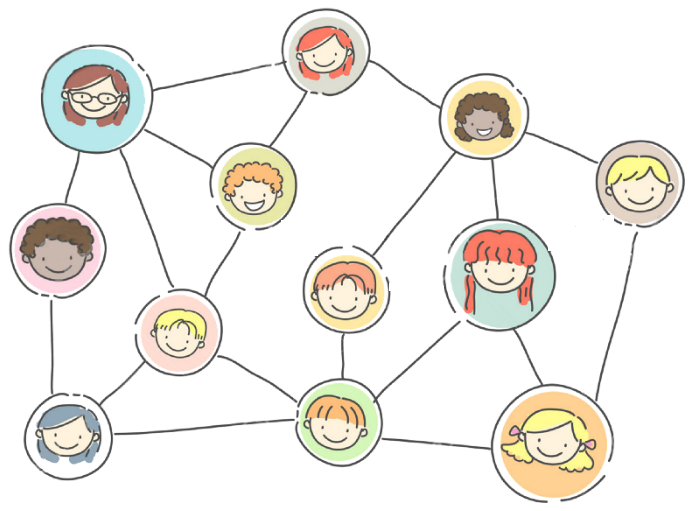
\includegraphics[scale=0.5]{Figuras/socialmedia.png}\\
Representação da relação entre pessoas numa rede social.

\end{ftst}

%=====

\begin{ftst}{Aplicações}{Teoria dos grafos}

\centering
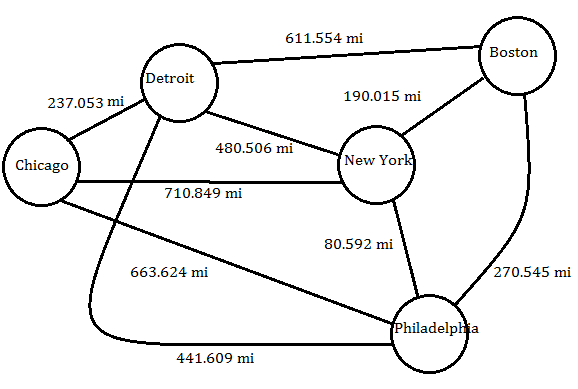
\includegraphics[scale=0.5]{Figuras/city.png}\\
Representação da ligação entre cidades e suas distâncias.
\end{ftst}

%=====

\begin{ftst}{Dígrafos}{Teoria dos grafos}
\justifying
Um \textbf{dígrafo} ou \textbf{grafo dirigido} consiste de um conjunto não vazio $V$ de vértices e um conjunto $E$ de arestas (que também podem ser chamadas de arcos), onde cada aresta é da forma $(v_i,v_j)$, sendo: $(v_i,v_j) \neq (v_j,v_i)$.
\vone
\vone
\centering
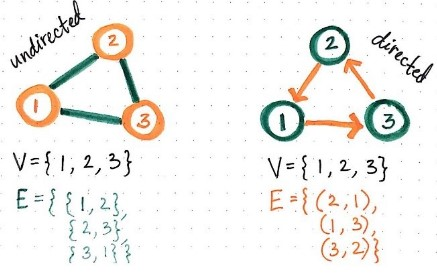
\includegraphics[scale=0.6]{Figuras/digrafo.jpg}\\

\end{ftst}

%=====

\begin{ftst}{Dígrafos}{Teoria dos grafos}
\centering
\textbf{Facebook x Twitter}

\vone
\justifying
Uma relação de amizade no Facebook pode ser facilmente representada como um grafo não direcionado, porque, se Ann é amiga de Bob, Bob também deve ser amigo de Ann. Não há direção, ambos são amigos um do outro.
\vone
\centering
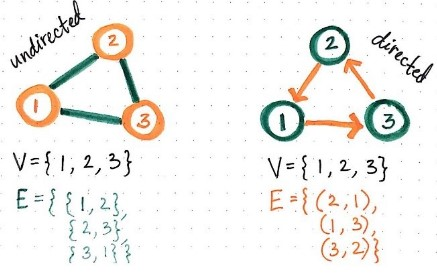
\includegraphics[scale=0.6]{Figuras/digrafo.jpg}\\

\end{ftst}

%=====

\begin{ftst}{Dígrafos}{Teoria dos grafos}
\centering
\textbf{Facebook x Twitter}

\vone
\justifying
Ao contrário do exemplo do Facebook, se Patrick segue Bob no Twitter, isso não exige que Bob siga Patrick de volta. Portanto, uma relação “seguir” deve ter um indicador de direção, mostrando qual vértice (usuário) tem uma aresta direcionada (segue) para o outro vértice.
\vone
\centering
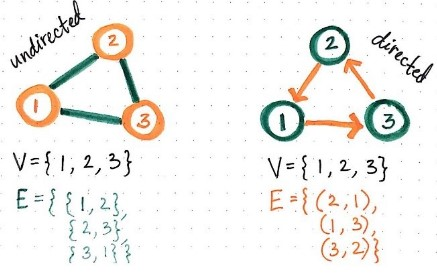
\includegraphics[scale=0.6]{Figuras/digrafo.jpg}\\

\end{ftst}

%=====

\begin{ftst}{Multigrafo}{Teoria dos grafos}
\justifying
Um \textbf{multigrafo} é um grafo que possui mais de uma aresta interligando os mesmos dois vértices (arestas múltiplas ou arestas paralelas). 
\vone
Formalmente, um multigrafo $G = (V,E,f$ é composto por um conjunto de vértices $V$, um conjunto de arestas $E$ e uma função $f$:
\vone
\vone
\vone
\centering
\huge
$f: \{E \rightarrow v_i, v_j \in V$ e $v_i \neq v_j \}$



\end{ftst}

%=====

\begin{ftst}
{Course Overview}
{Course Structure}
\begin{block}{Evaluation criteria}
	\begin{center}
		\small
		\begin{tabular}{cccc} \hline
			\textbf{Item}	& \textbf{Type}	&\textbf{Grades}\\
			\hline
			Case studies		& Short group projects		&35\\
			Written exam		& Written exam	&40\\
			Final Project		& Report and presentation		&25\\
			\hline
		\end{tabular}
	\end{center}
\end{block}

\begin{block}{Other relevant Information}
	\bitems Lectures slides, example R files, data, etc. available at \\
	{\small \url{http://git.io/v3Kh8}}
	\spitem Office hours: depends on the week. Please drop me a message to check availability.
	\spitem Software/services used: R ({\scriptsize\url{http://cran.r-project.org/}}),\\Github ({\scriptsize\url{http://github.com/}}).
	\eitem
\end{block}
\end{ftst}

%=====

\begin{ftst}
{Course Overview}
{Course Bibliography}
\textbf{Main}:\\
{\footnotesize
\bitems Felipe Campelo (2018), \textit{Lecture Notes on Design and Analysis of Experiments}. Online: \url{http://git.io/v3Kh8} Version 2.12; Creative Commons BY-NC-SA 4.0.
\item D.C. Montgomery, G.C. Runger (2010), \textit{Applied Statistics and Probability for Engineers}, John Wiley \& Sons.
\eitem}
\vhalf
\textbf{Additional}:
{\footnotesize
\bitems D.C. Montgomery (2012), \textit{Design and Analysis of Experiments}, Wiley.
\item Michael J. Crawley (2007), \textit{The R Book}, Wiley.
\item B. Caffo (2015), \textit{Statistical inference for data science}, LeanPub - {\small\url{https://leanpub.com/LittleInferenceBook/}}
\item J.J. Faraway (2002), \textit{Practical Regression and Anova using R} - {\small\url{http://goo.gl/ewMWL}}
\item D. Wiens (2005), \textit{Introduction to Design and Analysis of Experiments} - {\small\url{http://goo.gl/hZXg1}}
\eitem}
\end{ftst}

%=====

\begin{ftst}
{Course Overview}
{Required / Desired background}
This is a course on \textit{applied} experimental design and analysis. As such, a large portion of the course is dedicated to case studies in which the student will design experiments, collect (simulated) data, perform inference and report his or her analysis.
\vone
It is \textbf{strongly reccomended} that the student should complete the free online course  \textit{R Programming}\footnote{{\scriptsize\url{https://www.coursera.org/course/rprog}}} \textbf{before the end of the second week} of the semester (except if the student is already fluent in R).
\vone
It is also \textbf{strongly reccomended} that the student should complete the free online course  \textit{Reproducible Research}\footnote{{\scriptsize\url{https://www.coursera.org/course/repdata}}} \textbf{before the end of the first month} of the semester (except if the student is already capable of writing reports using R Markdown).
\end{ftst}

%=====

%\begin{ftstf}{About this material}{Conditions of use and referencing}
\centering\footnotesize This work is licensed under the Creative Commons CC BY-NC-SA 4.0 license\\(Attribution Non-Commercial Share Alike International License version 4.0).\\
\vhalf
\url{http://creativecommons.org/licenses/by-nc-sa/4.0/}\\
\vone
\footnotesize Please reference this work as:\\
\footnotesize \flushleft Felipe Campelo (2018), \textit{Lecture Notes on Design and Analysis of Experiments}.\\Online: {\scriptsize\url{https://github.com/fcampelo/Design-and-Analysis-of-Experiments}}\\
Version 2.12. Creative Commons BY-NC-SA 4.0.\\

\begin{Verbatim}[fontsize=\tiny]
    @Misc{Campelo2018,
      title={Lecture Notes on Design and Analysis of Experiments},
      author={Felipe Campelo},
      howPublished={\url{https://github.com/fcampelo/Design-and-Analysis-of-Experiments}},
      year={2018},
      note={Version 2.12. Creative Commons BY-NC-SA 4.0.},
    }
\end{Verbatim}

\begin{tikzpicture} [remember picture,overlay]
\node[anchor=south,yshift=0pt] at (current page.south){ \includegraphics[width=.2\textwidth]{../figs/CCsomerights.png}};
\end{tikzpicture}
\end{ftstf}

%=====

\end{document}